\documentclass[bachelor,english]{hgbthesis}

\usepackage{wrapfig}
\usepackage{listings}
\usepackage{tikz}
\usepackage{pgf-umlsd}
\usepgflibrary{arrows}
\usetikzlibrary{shadows}
\AddBibFile{literature.bib}

\begin{document}

\title{Hybrid Threads \\ for the \\ Parrot Virtual Machine}

\author{Stefan Seifert}
\studiengang{Software Engineering}
\studienort{Hagenberg}
\abgabemonat{Februar}
\abgabejahr{2012}

\nummer{1010307037-A}
\gegenstand{SWE}
\semester{Wintersemester 2012}
\betreuer{Dr. Heinz Dobler}
\license{This work is published under the conditions of the Creative Commons Attribution 3.0 Unported License (CC BY) -- see \url{http://creativecommons.org/licenses/by/3.0/}}

\frontmatter
\maketitle
\tableofcontents

\chapter{Acknowledgements}

I want to thank:
\begin{itemize}
\item{Andrew "whiteknight" Whitworth for laying the foundations for my work, being of tremendous help at all stages of the project and for fixing some of my bugs.}
\item{Nat "Chandon" Tuck for implementing the green thread basics on which my work is based on.}
\item{Christoph "cotto" Otto for bringing me into the Parrot project.}
\item{Brian "benabik" Gernhardt for lurking in the chat channel and at least trying to help with my many questions.}
\item{Markus "zimmski" Zimmerman for correcting many errors.}
\end{itemize}

\chapter{Abstract}

Parrot is a runtime system for dynamically typed programming languages. Despite several attempts in it's 10 years of history, it does not provide any support for multithreaded computation.

This thesis shows a way to implement threading support in Parrot using a hybrid approach using a combination of lightweight (``green'') threads and OS threads. These lightweight threads are used as messages in a system where reading shared variables is allowed but only the one owner thread may write to it. The implementation of this hybrid approach is described in detail and benchmarks are presented demonstrating the viability of this design.

\begin{german}
\chapter{Kurzfassung}

Parrot ist eine Laufzeitumgebung f{\"u}r dynamisch typisierte Programmiersprachen. Trotz mehrerer Anl{\"a}ufe in seiner zehnj{\"a}hrigen Geschichte, bietet Parrot keine Unterst{\"u}tzung f{\"u}r Multithreading.

Diese Arbeit zeigt einen Weg, um Threadingunterst{\"u}tzung in der Laufzeitumgebung zu implementieren mit Hilfe eines hybriden Systems aus leichtgewichtigen und Betriebssystem-Threads. Diese leichtgewichtigen Threads werden als Nachrichten in einem System benutzt, in dem das Lesen von gemeinsamen Daten erlaubt ist, aber nur der eine besitzende Thread darauf schreiben darf. Die Implementierung wird detailiert beschrieben und mit Benchmarks die Brauchbarkeit des Designs gezeigt.

\end{german}

\mainmatter

\chapter{Introduction and Motivation}

%
On July 19th 2000, the Perl 6 design process was announced. Perl 5 had been a flexible and widely used programming language but had started to show its age and suffered from early design decisions.

Am example of Perl:
\begin{GenericCode}
use common::sense;

my @friends = qw(Ann Bob);
say "Hello $_" foreach @friends;
\end{GenericCode}


The Perl interpreter is written in C and has accumulated a lot of cruft over the years. The general consensus among the core developers was that the code had reached a state where maintenance was approaching impossibility \cite{Masak40451}. An attempt to reimplement these internals had failed but led to the decision that the interpreter for a Perl 6 language should be developed independently of the needs of Perl 5. Since the Perl 6 syntax was very much in flux (and parts of it still are) the designers of these new internals tried to work very independently of any syntax related questions \cite{Developer}. Taking up the name born in an April Fool's Day joke announcing the merging of the Perl and Python programming languages, these new internals were called Parrot \cite{Perl}.

Parrot evolved from being just the interpreter for the new version of Perl to being a language independent VM providing features like garbage collection, exception handling and dynamic typing. At the time when the Parrot project started, the Java and .NET VM were widely used, but both targeted statically typed languages. Parrot thus filled a quickly growing niche.

The Perl 6 design process began with asking the Perl users what they were expecting from the new version of the language. The very first feature that got asked for was well integrated multithreading support \cite{RFC1}. Perl 5 had two different implementations of thread support. In the first model, called \textit{5005threads}, data was shared by default and shared access to data had to be explicitly synchronized. This was similar to the models used by languages such as C or Java. The implementation however suffered from data corruption and crashes and thus was not recommended for production use \cite{ThreadManual}. Perl 5.6 introduced the newer model called \textit{ithreads}, mostly as a way to emulate \textit{fork} on Win32 platforms. Perl 5.8 exposed this Application Programming Interface (API) to the user of the programming language. In this new model, all data is copied to each thread and afterwards thread local. Data must be explicitly shared between threads.

In other words, in Perl threads are not lightweight at all. They have severe impact on memory usage, writes to shared variables are expensive and still not all features of the language are usable in threaded programs.

Being born at a time when Perl 6 still looked much more similar to Perl 5 than it does nowadays, Parrot's threading support initially was very close to Perl's \textit{ithreads} model. Previous attempts to change this into the more conventional model of data shared by default or implementing new technologies like \textit{Software Transactional Memory} failed. For example Parrot has never supported running multiple threads and having garbage collection at the same time.

\section{Why is multithreading support so important?}

In the year 2005 development of faster Central Processing Units (CPUs) shifted from increased speed of a single core to adding more cores. Modern processors contain up to 12 cores with even mobile phones having up to four. To utilize a modern CPU's power, code needs to be run in parallel. In UNIX (and thus Perl) tradition, this is accomplished using multiple processes being a good solution for many use cases. For many others like auto threading of hyper operators in Perl 6, the cost of process setup and communication would be prohibitively high except for very large data sets.

\section{Why is multithreading support so difficult to implement?}

Low level programming languages like C provide only the bare necessities, leaving the responsibility for preventing data corruption and synchronization entirely to the user. A high-level language like Perl 6 on the other hand provides complex and compound data types, handles garbage collection and a very dynamic object system. Even seemingly simple things like a method call can become very complex. In a statically typed programming language the definition of a class is immutable. Thus, calling a method on an object contains just the steps of determining the object's class, fetching the required method from this class and calling it. Calling the same method again can then even omit the first two steps since their results cannot change.

In a dynamic language, the object may change its class at runtime. The inheritance hierarchy of the class may be changed by adding or removing parent classes. Methods may be added to or removed from classes (or objects) at runtime and even the way how to find a method of a class may change. So a simple method call results in the following steps:
%
\begin{itemize}
\item determining the class of the object,
\item determining the method resolution method of the class,
\item finding the actual method to call,
\item calling the method.
\end{itemize}
%
These steps have to be repeated for every method call, because the results may change any time. In a threaded environment, a thread running in parallel may change the underlying data and meta data in between those sequences and even between those steps. As a consequence, this meta data has to be protected from corruption introducing the need for locks in a performance critical area.

Many interpreters for dynamic languages like Python \cite{LearningPython} or Ruby \cite{TheRubyProgrammingLanguage} handle this problem by using a global interpreter lock to effectively serialize all operations. This is a proven and reliable way but leaves much of the hardware's potential unused.

\section{Current status}

During the years of back and forth and failed attempts of adding threading support to Parrot, the Perl 6 specification evolved to a point where the largest parts of the language were covered and its features were implemented in the compilers. The lack of concurrency primitives in Parrot however prevents any progress in the area of concurrency support.

Before the work on this thesis started, Parrot did not have any threading support at all. The previous, defunct implementation had been removed.

This thesis suggests a new approach based on a hybrid threading system. So called \textit{green threads} are used to simplify the implementation of a nearly lock free multithreading implementation. This approach is based on a design by Andrew Whitworth and Nat Tuck \cite{WKnightThreading}. The goal of this thesis is to demonstrate the advantages of this model and produce a working implementation which can be used to investigate the performance characteristics of a hybrid threading system.

\chapter{Concurrency in other Programming Platforms}

This chapter is about programming platforms. A platform is seen as a combination of a programming language and a runtime. E.g. for the Python programming language there are multiple runtimes with different implementations of threading support.

\section{Java}

In Java, the user is responsible for preventing concurrency issues. The language provides synchronization primitives like mutexes, but the interpreter (the Java Virtual Machine, JVM) does not protect the consistency of the provided data structures. The class library provides the user with high-level data structures explicitly designed for multithreaded scenarios.

Java version 1.1 used \textit{green threads} to support multithreaded execution of Java programs. Green threads are threads simulated by the virtual machine (VM) but unable to use more than one CPU core for processing. Details are described in chapter~\ref{cha:green_threads}. Version 1.2 introduced native Operating System (OS) threading support which since has become the standard way to do multithreading in Java \cite{JavaThreadManual}.

Following is an example of a multithreaded program in Java. The program spawns 10,000 threads, each one waiting for the \textit{starter} variable to be set to 1 before adding it's name to an array:
\begin{JavaCode}
import java.util.Vector;
import java.util.ArrayList;

class ThreadingExample {
    private static Vector<Integer> results = new Vector<Integer>();
    private static int starter = 0;

    private class Sayer extends Thread {
        private int name;

        public Sayer(int name) {
            this.name = name;
        }

        public void run() {
            while (starter == 0) {
                try { Thread.sleep(100); } // milliseconds
                catch(InterruptedException e) { }
            }

            results.add(name);
        }
    }

    public static void main(String args[]) {
        ThreadingExample e = new ThreadingExample();
        e.test();
    }

    private void test() {
        ArrayList<Thread> threads = new ArrayList<Thread>();

        for (int i = 0; i < 10000; i++) {
            Thread t = new Sayer(i);
            t.start();
            threads.add(t);
        }

        starter = 1;

        for(Thread t: threads)
            try { t.join(); }
            catch(InterruptedException e) { }

        System.out.println(results.size());
    }
}
\end{JavaCode}


The program exploits the fact that all methods in the \textit{Vector} class are synchronized, i.e. thread-safe. If the \textit{results} array was a non-thread-safe \textit{ArrayList} instead, access would have to be locked manually:

\begin{JavaCode}
synchronize(results) {
    results.add(name);
}
\end{JavaCode}

\section{Python}

Python provides threading support through the \textit{threading} module.

The CPython implementation of the Python runtime uses a \textit{Global Interpreter Lock} (GIL) to protect its internal consistency \cite{PythonThreadingManual}. This is a single lock taken whenever the interpreter executes Python bytecode. Because of this lock, only one thread can execute bytecode at any time so all built-in types and the object model are implicitly type safe. The drawback is that Python code cannot benefit from having multiple CPU cores available. However I/O operations and calls to external libraries are executed without holding the GIL, so in applications with multiple I/O bounded threads, there may still be a performance benefit from using multithreading.

To run Python code in parallel, multiple processes have to be used. The \textit{multiprocessing} module provides support for spawning processes exposed through an API similar to the \textit{threading} module \cite{PythonMultiProcessingManual}. Since processes may not directly access other processes' memory, the \textit{multiprocessing} module provides several means of communication between processes: \textit{Queues}, \textit{Pipes} and shared memory support.

Following is an example of a multithreaded program in Python. The program spawns 10,000 threads, each one waiting for the \textit{starter} variable to be set to 1 before appending it's name to an array:
\begin{GenericCode}
from threading import Thread
from time import sleep

starter = 0
results = []
threads = []

def sayer(name, results):
    while starter == 0:
        sleep(0.1)
    results.append(name)

for i in range(10000):
    t = Thread(target = sayer, args = (i, results))
    t.start();
    threads.append(t)

starter = 1

for t in threads:
    t.join()

print len(results)
\end{GenericCode}


Even though many threads append to the same array, they do not have to take any locks. The GIL implicitly protects the array by allowing only one Python instruction to be run at any time.

\chapter{Parrot}

Parrot consists of the VM (also called interpreter), and various tools to facilitate the implementation of programming languages on top of the Parrot VM (the \textit{Parrot Compiler Toolkit}). This thesis concentrates on the VM itself. The interpreter is written in C. Example code and test cases are written in \textit{Parrot Intermediate Representation} (PIR) a high-level assembly language abstracting register allocations and function calling conventions.

Contrary to other widely used VMs like the JVM or the \textit{Common Language Runtime} (CLR) which are stack based, Parrot mirrors contemporary hardware CPUs more closely by being register based. A stack based VM usually pops the operands for an operation from the top of a stack and pushes the result back. Thus the operands are chosen implicitly by ordering of the operations allowing the opcodes to be without operands. In a register based VM on the other hand, each operation has to specify the operands explicitly. Compilers for stack machines are simpler because they do not have to care about register allocation and code is independent of prior or subsequent code \cite{VMShowdown}. The rationale behind giving up the simplicity of a stack based implementation is the hope of simplifying just-in-time (JIT) compilation and improved performance of nested function and method calls.

The current design of Parrot uses four sets of registers where each one has an unlimited number of registers. The four sets are correspondingly to Parrot's types:
%
\begin{itemize}
\item integer,
\item floating point,
\item string and
\item polymorphic container (PMC).
\end{itemize}

The first three register types are self explanatory. String in Parrot is a low-level type with the interpreter handling all memory allocation issues and Unicode encoding. String values are immutable.

\section{\textit{PolyMorphic Containers} (PMCs)}
\label{sec:PMCs}

PMCs are containers for all high level types such as objects, arrays, hash tables or code. Thus, they are similar to Python's \textit{PythonObject} types. PMCs are defined by C structs and are garbage collected. Their definition looks like:
\begin{CCode}
struct PMC {
    Parrot_UInt    flags;
    VTABLE         *vtable;             /* Pointer to vtable. */
    DPOINTER       *data;               /* Pointer to attribute structure. */
    PMC            *_metadata;          /* Pointer to metadata PMC. */
};
\end{CCode}
In short, they contain a pointer to a type specific data structure and some meta data. The \textit{vtable} is a virtual method table, where the type's behavior is defined. It contains a list of function pointers forming Parrot's unified type interface. This interface is a union of numeric, string, array, hash and object like behaviors. For example the  \textit{get\_integer} function returns an integer value for the data type. For a simple \textit{int} it is the value. For an array it may be the number of elements. The \textit{find\_method} function makes user defined methods of objects possible.

In this way, a language implementer can define the basic types of the language and available operations on them. For each \textit{vtable} entry, there is a corresponding opcode in Parrot's bytecode. Thus an \textit{inc \$P0} instruction calls the \textit{increment} vtable function of the PMC pointed to by the \textit{\$P0} register.

PMCs are implemented in \textit{pmc} files with method bodies written in C. These files are preprocessed to plain C before compilation.

\section{\textit{ParrotInterpreter}}

The Parrot interpreter is represented by a C struct called \textit{parrot\_interp\_t}. This structure contains pointers to the garbage collector's runtime data, the loaded types, vtables, the runloop, the current continuation and other global data. A pointer to this structure is passed to almost every function as the first parameter.

There is also the \textit{ParrotInterpreter} PMC which exposes parts of the \textit{parrot\_interp\_t} struct to the user.

\section{Continuation passing}

Control flow in Parrot is modeled using continuation passing. A continuation is a data structure containing the state of a program at a given point in its execution. It contains all information necessary to continue a program in a certain state, e.g. a call stack, the instruction pointer and contents of local variables. Calling a continuation means restoring the state encapsulated in the continuation.

When a function is called, instead of pushing a return address on the stack, the function is given a return continuation as part of its parameters. Returning from a function means calling the return continuation with possible return values stored in the registers where the calling code is expecting them. Continuation passing makes things like tail call optimization\footnote{When in the last statement of a function another function is called and its value returned unchanged, the outer function can just pass on its return continuation thus saving the need to create a new continuation and one step on returning from the nested function.} simple and as described in chapter~\ref{cha:green_threads} is a important part of implementing green threads.

\section{Runloops}
\label{sec:Runloops}

A runloop is the inner most loop executing bytecode in Parrot. It consists of two steps as shown in the following pseudo code:
\begin{GenericCode}
while (pc != NULL) { // program counter points to an opcode
    op = fetch_opcode_at(pc);
    pc = execute_opcode(op);
}
\end{GenericCode}

\begin{figure}
\centering
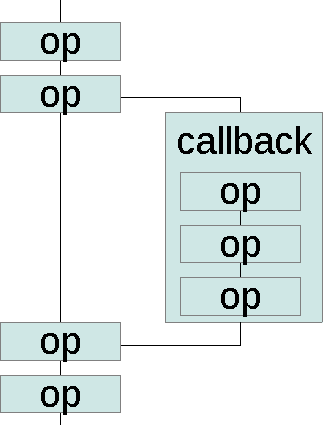
\includegraphics[scale=.4]{runloops}
\caption{Example of a callback executing in a nested runloop.}
\label{fig:runloops}
\end{figure}

It is also a data structure containing information needed to support exception handling. When some operation in Parrot bytecode is calling a C function and this C function in turn is again executing Parrot bytecode, a nested runloop is started. Examples for such situations include calling a library function with a callback as parameter and exceptions thrown inside Parrot's C code calling a previously defined exception handler in user code. This is shown in figure~\ref{fig:runloops}.

\section{Exception handling}

Before entering a runloop, the \textit{setjmp} C function is used to save the current stack position and register contents in a data structure stored in the runloop meta data. This is effectively creating something resembling a continuation at the C level. When an exception is created within the interpreter, the runloop stack is searched for the runloop containing a suitable exception handler. \textit{longjmp} is then used to unwind the call stack up to the point where \textit{setjmp} was called and the call environment is restored. While having great similarities with continuations, this mechanism is more limited. It only allows to jump back to a point ``higher'' in the call stack.

\section{Garbage Collector (GC)}

Parrot supports different Garbage Collector (GC) implementations which can be selected at interpreter startup. Currently, there are four implementations of different algorithms:
\begin{itemize}
\item Inf: a GC for debugging purposes never collecting any garbage.
\item MS: a basic mark and sweep implementation.
\item MS2: a non-recursive mark and sweep implementation.
\item GMS: a generational, non-compacting, mark and sweep GC.
\end{itemize}
GMS is the default.

A mark and sweep GC operates in two phases: In the mark phase, starting from a known root set of objects, the GC follows pointers in the object graph, marking each encountered object as alive. In the sweep phase, all objects not being alive are destroyed and all the live flags are reset.

In a process with many objects, having to traverse the whole graph may take a considerable amount of time. To mitigate this, a generational GC extends this algorithm by assuming that the longer an object is alive, the lower the chances are that it will become unused. So, the objects are partitioned into different generations. The youngest generation will always be traversed while the older generations will be handled much less frequently or even never more at all.

\section{Historical development}

Much of Parrot's previous threading related code has been removed to clean up the code and improve performance. Since the existing threading support was known to be unreliable and seriously flawed, this was no trade off. The final parts were removed by the merging of the \textit{kill\_threads} branch on September, 21st 2011.

In 2010, Nat Tuck began working on a \textit{green\_threads} branch during his Google Summer of Code internship. The feature got prototyped using pure PIR and then implemented in Parrot's core. He got it to work in simple cases and started to work on OS thread support but the internship ended before the code was ready to be merged into the master branch. The code lay dormant until the work on this thesis started in 2011.

\chapter{Green threads}
\label{cha:green_threads}

Green threads are one way to model concurrent control flows in a program. To get a better understanding of what they are and how they work, the possible options for supporting concurrency are discussed before explaining green threads in detail.

\section{Coroutines}

Coroutines are functions retaining their state between calls. Instead of returning, they yield control back to the calling function, possibly with an intermediate result returned. A very simple example in Python looks like:
\begin{GenericCode}
def counter():
    for i in range(0, 100):
        yield i
\end{GenericCode}
This function returns one integer for every call, counting from 0 to 100. An example usage looks like:
\begin{GenericCode}
def count\_up():
    x = counter()
    print x
    x = counter()
    print x
\end{GenericCode}
This example prints the numbers 0 and 1. For the two functions to run in parallel, they have to cooperate. One by calling the other repeatedly and the callee by yielding control back to the caller.

\section{Operating system threads}

OS threads are like multiple processes running in parallel but share their memory. The OS is responsible for giving each of these threads CPU time to run. OS threads are the only option where more than one thread may be executed by the CPU(s) at the same time if the hardware permits.

\section {Green threads}

\textit{Green threads} or \textit{lightweight threads} are threads managed by the VM instead of by the OS. For better distinction green threads are henceforth referred to as \textit{tasks}. These tasks only run pseudo parallel. The VM has a scheduler and support for preempting running tasks.
Preemption means to suspend a task regardless of what it is currently doing and probably resuming it later on.
This is an implementation of the many-to-one threading model very similar to what an OS running on a system with a single CPU core does.
%
Advantages of green threads are:
%
\begin{itemize}
\item They allow pseudo concurrent processing without endangering the interpreter's internal consistency.
\item Green threads are light weight having low memory overhead and close to zero creation time.
\item They do not depend on OS threading support.
\item The interpreter controls the point of preemption of a green thread.
\item The interpreter controls the scheduling policy and may allow the user to influence it or even take over completely.
\item Garbage collection can be implemented like in a singlethreaded process.
\item Critical sections can be protected by disabling the scheduler until the code is clear of the section.
\end{itemize}
%
Disadvantages include:
%
\begin{itemize}
\item Green threads do not allow more than one CPU core to be used for computations.
\item Blocking calls like I/O block the interpreter including other green threads.
\item The interpreter has to provide logic and timers to control green threads.
\end{itemize}

Green threads differ from coroutines in that the interpreter decides when a running task is to be preempted while a coroutine depends on explicit yield calls.

Below is an example in order to explain why concurrent processing can endanger the interpreter's internal consistency. The basic problem are concurrent writes to shared variables. Assuming an implementation of an array class consisting of the field holding the data and the number of contained elements in a separate member variable:
\begin{CCode}
pmclass ResizableIntegerArray auto_attrs provides array {
    ATTR INTVAL   size;      /* number of INTVALs stored in this array */
    ATTR INTVAL * int_array; /* INTVALs are stored here */
\end{CCode}
To append a new value, the array has to read the current size, write the new value at the position \textit{size} + 1 and then write the incremented size back into the member variable.
Now, if two threads simultaneously try to do this, it may happen that both read the same size, write to the same position (with one overwriting the value of the other) and write back the same incremented size. In this case one of the appended values is lost.

In a more complicated example, the array could have to resize its data buffer to accept the new value. It would read the current size, allocate a new buffer, copy the values to the new buffer and then destroy the old one. Again, if two threads try to do this simultaneously, one of them could still be copying data, while the other already destroys the old buffer. This leads to the copying thread accessing freed memory.

When garbage collection is brought into the mix, the possibilities for corruption grow even further. At the point where the first thread needs to allocate the new buffer, the GC could decide that it needs to clear some unused memory. It would have to traverse the object graph to mark alive objects. Between the mark and the sweep phases, the second thread could change the pointer to the buffer from the old one to the new one. So the old buffer would have been marked alive, while during the sweep phase the new buffer would be in its place, but not yet marked alive.

\section{Green threads in Parrot}

Parrot's green threads implementation is based on Nat Tuck's \textit{green\_threads} branch developed during his Google Summer of Code internship \cite{ChandonBlog}.

In Parrot, green threads are called \textit{Tasks}. Each task is assigned a fixed amount of execution time. After this time is up a timer callback sets a flag which is checked at execution of every branch operation. Since the interpreter's state is well defined at this point, its internal consistency is guaranteed. The same holds for the GC. Since task preemption is only done while executing user-level code, the GC can do its work undisturbed and without the need for measures like locking. Since user-level code is allowed to disable the scheduler, it can be guaranteed to run undisturbed through critical sections.

The scheduler is implemented as a PMC type. This allows the user to subclass this PMC thus allowing fine-grained control over the scheduling policy. Features, a user could add this way would be for example giving different priorities to tasks or implementing the possibility to suspend and resume a task.

\chapter{Design of Hybrid Threads}
\label{cha:design}

This chapter describes how green threads are used to solve the following problems occurring when trying to implement threading support:
%
\begin{itemize}
\item How to ensure internal interpreter consistency when doing writes to shared variables?
\item How to implement critical sections?
\item How to handle GC?
\end{itemize}

In keeping the analogy of the interpreter being a software CPU, multithreading is implemented by having a separate interpreter with its own register set for each thread. Thus the words \textit{thread} and \textit{interpreter} are used interchangeably as there is a 1:1 relationship between them. When a user starts a new task, the scheduler first looks for an idle thread. If one can be found, the task is scheduled on the thread's interpreter. If none can be found, a new thread with a new interpreter is started. Parrot tries to optimize the number of utilized threads by creating at most one for each CPU core in the system. If more tasks are started than the maximum number of threads, the tasks are distributed evenly among the running interpreters. This is effectively an implementation of the N:M threading model.

\section{Shared data}

As described in the introduction, cross-thread writes to shared variables may endanger the internal consistency of the interpreter. Traditionally, the solution to this problem is the use of locks of varying granularity. Fine-grained locking allows code to run in parallel but taking and releasing locks costs performance. It not only increases the instruction count and memory accesses but it also forces the CPU cores to coordinate and thus communicate. Even a seemingly simple operation like an atomic increment can take two orders of magnitude longer than a normal increment \cite{LockingInOSKernels}. While the gain through being able to utilize multiple CPU cores may offset this cost, it is still impacting the common case of having only a single thread running.

Too coarse locking on the other hand would reduce scalability and the performance gains through parallel execution by having threads wait for extended periods for locks to become available. In the extreme case of having a global interpreter lock it would effectively serialize all computations costing much of the benefits of using threads in the first place.

The other problem with locking is the possibility of introducing deadlocks. For example, two functions \textit{F1} and \textit{F2} both use two resources \textit{A} and \textit{B} protected by locks. If \textit{F1} first locks \textit{A} and then tries to lock \textit{B} while \textit{F2} has already locked \textit{B} and is now trying to lock \textit{A}, the program would come to a halt. Both functions would be left waiting for the other to unlock the resource which will never happen. With fine-grained locking, the possibilities for such bugs grow quickly. At the same time, it is easy to miss a case where a lock would be appropriate leading to difficult to diagnose corruption bugs.

The solution for these problems implemented in this thesis is to sidestep them altogether by disallowing write access to shared variables. The programmer (or in most cases the compiler) is obliged to declare a list of all shared variables before a newly created task is started. The interpreter would then create proxy objects for these variables which the task can use to access the data. These proxies contain references to the original objects. They use these references to forward all reading \textit{vtable} functions to the originals. Write access on the other hand would lead to a runtime error.

In other words, all data is owned by the thread creating it and only the owner may write to it. Other threads have only read access.

For threads to be able to communicate with their creators and other threads, they still need to write to shared variables. This is where green threads come into play. Since green threads are light weight, it is feasible for a thread to create a task just for updating a variable. This task is scheduled on the interpreter owning this variable. To reduce latency, the task is flagged to run immediately. The data-owning interpreter will preempt the currently running task and process the new write task. Put another way, the data-owning interpreter is told what to write to its variables, so other threads don't have to.

\begin{figure}
    \centering
    \begin{sequencediagram}
        \newthread{main}{:MainThread}
        \newinst{shared}{:A}
        \newthread{child}{:ChildThread}

        \begin{callself}{main}{task1}{}
        \end{callself}

        \prelevel\prelevel
        \begin{callself}{child}{task2}{}
            \postlevel
            \begin{messcall}[1]{child}{schedule(write\_task)}{main}
                \begin{callself}{main}{write\_task}{}
                    \begin{messcall}{main}{write}{shared}
                    \end{messcall}
                \end{callself}
            \end{messcall}
        \end{callself}

        \prelevel\prelevel
        \begin{callself}{main}{task1}{}
        \end{callself}

    \end{sequencediagram}
    \caption{\textit{task2} running on \textit{ChildThread} is sending the \textit{write\_task} to the \textit{MainThread} to write to the shared variable \textit{A}.}
    \label{fig:hybridthreads}
\end{figure}

\section{Critical Sections}

Critical sections can be implemented by disabling preemption until the code has left the section. With other threads not being allowed to write to the data and the current task running uninterrupted it it guaranteed to complete without the data being changed from outside.

\section{Garbage Collection (GC)}

A GC has to traverse and process the entire graph of objects in memory. If during this traversal another thread is changing this structure by creating new objects, moving them around in the graph or removing them, the GC's data would be compromised. For example, it could happen that the GC does not mark referenced objects alive because they were added to objects which have already been processed.

In previous attempts to implement threading support in Parrot, the solution to this problem was to disable the GC while multiple threads were active. While multithreaded GC algorithms exist, their implementation would have been too complex and brittle for this thesis \cite{VCGC}. Other VMs solve this problem by suspending all threads while the GC is running. Suspending all threads is not as simple as it sounds because these threads can be in any state at the time. For example, they could be blocking on some long running I/O operation like waiting for a reply on a network connection. A thread can stay in this condition indefinitely thereby never being able to confirm synchronization.

Since cross-threaded writes are already forbidden and all read access to other thread's data goes through the narrow channel of proxy objects, forcing a complete separation of the thread's memory domains is only a small step. By having separate memory areas for each interpreter, it becomes possible to have each interpreter run its own GC. This way, the known to work singlethreaded GC implementation can be used nearly unchanged.

With separated memory domains, it can happen that an object is created on one thread, used on another thread but not any more on the owner thread. Without any additional measures, the GC would collect such objects, since it does not know about references from other threads. But since all objects which could be accessed from other threads have to be pushed onto the task object representing these threads, the objects can still be referenced from the task object. Since the task is still owned by the original thread, the GC knows that these objects are still in use.

\chapter{Implementation of Hybrid Threads}

\section{Scheduler}

The scheduler is the place where most of the green thread logic is implemented. It consists of two parts: functions using the prefix \textit{Parrot\_cx} which are located in \textit{src/scheduler.c} and the scheduler PMC type containing the scheduler's data and public interface.

\textit{Parrot\_cx\_init\_scheduler} is called from \textit{Parrot\_interp\_initialize\_interpreter} whenever a new interpreter is created, e.g., on interpreter startup and whenever a new thread is created. It creates the scheduler PMC and sets up alarm signal handling.

The scheduler is hooked into the system by replacing the call to execute the \textit{main\_sub} by a call to \textit{Parrot\_cx\_begin\_execution}. The latter creates the main task using \textit{main\_sub} as the task's code. This task is then put onto the run queue. The scheduler timer gets enabled and control is given to \textit{Parrot\_cx\_outer\_runloop}.

\textit{Parrot\_cx\_outer\_runloop} is the loop taking tasks from the run queue and executing them. Despite its name, it may not be confused with runloops discussed in section~\ref{sec:Runloops}. \textit{Parrot\_cx\_outer\_runloop} actually consists of two nested loops. The inner loop fetches tasks from the task queue and executes as long as tasks are available. Even when all tasks are finished there may still be alarms pending which upon termination would trigger new tasks to be scheduled. For this reason, there is an outer loop checking for pending alarms. If it finds any it puts the thread to sleep until the next alarm expires.

\textit{Parrot\_cx\_next\_task} contains the code to take the next task from the run queue and executing it. Before calling the task, it checks if there are other tasks still in the queue. Only if other tasks are waiting, task preemption is enabled. Otherwise, the current task will run until it finishes by itself, schedules other tasks or an alarm expires. This is an optimization reducing the runtime overhead of green threads in the important single tasking case to zero.

To enable task preemption, \textit{Parrot\_cx\_enable\_preemption} sets a flag on the scheduler PMC and uses \textit{Parrot\_cx\_set\_scheduler\_alarm} to set an alarm at a point in time \textit{PARROT\_TASK\_SWITCH\_QUANTUM} milliseconds in the future.

When an alarm is triggered, Parrot only increments the global \textit{alarm\_serial}. This serial is checked for changes by \textit{Parrot\_alarm\_check} being called by \textit{Parrot\_cx\_check\_scheduler}. This function in turn is called once for every \textit{branch} operation. When the serial is different from the last check or the \textit{SCHEDULER\_wake\_requested} flag is set, \textit{Parrot\_cx\_check\_scheduler} wakes up the scheduler by calling \textit{Parrot\_cx\_run\_scheduler}.

Since POSIX alarms can only be delivered to the main thread of a process, \textit{Parrot\_cx\_run\_scheduler} uses \textit{Parrot\_thread\_notify\_threads} to relay alarms to other thread's schedulers. For this purpose, every thread has a pipe which \textit{Parrot\_thread\_notify\_threads} writes a dummy byte to. The next step for the \textit{Parrot\_cx\_run\_scheduler} is to check for any expired alarms using \textit{Parrot\_cx\_check\_alarms}. An alarm has a task as callback. On expiry, this callback gets scheduled for immediate execution. As alarm signals do not contain any information about their origin, the scheduler does not know if the alarm was scheduled by user code or if it is the scheduler's preemption alarm. \textit{Parrot\_cx\_check\_quantum} is therefore used to check if the current task has used its assigned quantum and if it should be preempted.

Preemption of a task is implemented in \textit{Parrot\_cx\_preempt\_task}. It uses \textit{Parrot\_cx\_stop\_task} to create a continuation at the current point of execution and store it as the task's code. The task itself is then appended at the end of the run queue. The function returns a \textit{NULL} opcode which is propagated all the way up through the stack back to the \textit{branch} operation checking for alarms. The operation then recognizes this as the signal to stop processing and to exit the runloop.

The control flow ends up back at \textit{Parrot\_cx\_next\_task} at the point after executing the task. \textit{Parrot\_cx\_next\_task} then returns to \textit{Parrot\_cx\_outer\_runloop}.

The \textit{schedule} opcode is used to schedule a new task from user code. It uses \textit{Parrot\_cx\_schedule\_task} which starts new worker threads if needed and possible and pushes the task on the target thread's scheduler's task queue. If the target thread previously was executing only a single task, its preemption has been disabled for optimization as described above. So in this case \textit{Parrot\_cx\_schedule\_task} has to enable preemption to give the new task a chance to run.

\textit{Parrot\_cx\_schedule\_immediate} is used in various places like at alarm expiry for putting a task at the head of the run queue and immediately causing preemption of the currently running task. It does this by setting \textit{SCHEDULER\_wake\_requested} and \textit{SCHEDULER\_resched\_requested} flags the same as when the preemption alarm expires. To be precise, this mechanism leads to the current task being preempted at the next \textit{branch} operation since this is the place where the mentioned flags will be checked.

Alarms can be registered using \textit{Parrot\_cx\_schedule\_alarm}. It puts the alarm in the appropriate place in the ordered alarm list and uses \textit{Parrot\_alarm\_set} which sets the actual alarm but only if there is not another alarm already set for an earlier time, since there can only be one POSIX alarm pending at any time.

\textit{Parrot\_cx\_schedule\_sleep} is the actual implementation of the \textit{sleep} op. Like in \textit{Parrot\_cx\_preempt\_task}, \textit{Parrot\_cx\_stop\_task} is used to get an updated task at the current execution position, but instead of pushing this on the run queue, it is used as a callback for a newly set alarm. Again, the \textit{NULL} opcode is used to stop processing of the current task.

\section{Scheduler PMC}

The Scheduler PMC contains the following attributes:
%
\begin{itemize}
\item \textit{PMC *task\_queue}: list of tasks/green threads waiting to run.
\item \textit{Parrot\_mutex task\_queue\_lock}: a lock protecting the task\_queue so other threads can access it safely.
\item \textit{PMC *alarms}: list of future alarms ordered by time.
\item \textit{PMC *all\_tasks}: hash of all active tasks by ID.
\item \textit{UINTVAL next\_task\_id}: ID to assign to the next created task.
\item \textit{Parrot\_Interp interp}: a reference to the scheduler's interpreter.
\end{itemize}

\textit{push\_pmc} and \textit{unshift\_pmc} are used to add a task at the end, respectively the beginning of the task\_queue. \textit{shift\_pmc} is used to fetch and remove a task from the tip of the \textit{task\_queue}. \textit{get\_integer} returns the number of tasks in the \textit{task\_queue}. These four methods use the \textit{task\_queue\_lock} to make accessing the \textit{task\_queue} thread safe. Thus, the Scheduler PMC acts as a container while using \textit{task\_queue} to actually store the data.

\textit{alarms} is list containing all pending alarms, sorted by their expiration time. Sorted insertion is used to keep alarms in order. Sorting makes it simple and efficient to retrieve all alarms that have expired at a certain point in time.

The \textit{active\_tasks} returns an array containing all tasks which have been run at least once and are not yet finished, e.g., they are currently being executed or are preempted.

\section{Task PMC}

The Task PMC contains the following attributes:
%
\begin{itemize}
\item \textit{UINTVAL id}: Unique identifier for the task.
\item \textit{FLOATVAL birthtime}: the creation time stamp of the task.
\item \textit{Parrot\_Interp interp}: the interpreter which created the task.
\item \textit{PMC *code}: the code to run.
\item \textit{PMC *data}: additional data for the task given as parameter to \textit{code}.
\item \textit{INTVAL killed}: flag marking killed tasks.
\item \textit{PMC *waiters}: tasks waiting on this one.
\item \textit{PMC *shared}: list of variables shared with this task.
\item \textit{PMC *partner}: copy of this task on the other side of a GC barrier, meaning in another thread.
\end{itemize}

The \textit{invoke} method is used to run the task. It first checks the \textit{killed} flag to see if the task has been killed while waiting in the task queue. Parrot manages a \textit{recursion depth} counter which records, how many levels the call stack has. This counter is incremented by \textit{Parrot\_Sub\_invoke} for each call to a subroutine and decremented when a subroutine returns. While \textit{Parrot\_Sub\_invoke} is used to start or resume a task, the executed subroutine does not return when the task is preempted. This leads to \textit{recursion depth} growing until a \textit{recursion depth exceeded} exception is thrown. Therefore, as a workaround, the current \textit{recursion depth} is saved to a local variable and restored when the task stops executing.

The next steps are to add the task to the list of active tasks and to invoke the task's \textit{code}. \textit{data} is an optional parameter to the subroutine given as \textit{code}. Since this can be a compound object, a single parameter can cover all use cases.

If the task has been killed while being in the task queue or while running or it just ended, it gets removed from the list of active tasks and all tasks registered with this task's \textit{waiters} array are added to the scheduler's task queue to be run.

\textit{push\_pmc} and \textit{pop\_pmc} are used to add or remove variables to the task's list of shared variables. For these variables, proxies will be created when the task is run on a different thread.

The \textit{kill} method is used to set the task's \textit{killed} flag.

\section{Runloops}

Runloops are created whenever a part of Parrot's C internals starts to execute bytecode. This can be at interpreter startup to start the actual program execution or when some library function needs to execute a user callback. An exception handler can also be such a callback. Each runloop has a unique id. These ids are numbered from 0 and increased by 1 whenever a new runloop is created.

When an exception is thrown, Parrot searches for a previously set up exception handler and executes it. As part of exception handling finalization, it cleans up, freeing any information no longer needed. The exception handler does not have to have been set up in the same runloop from which the exception has been thrown. Parrot uses the runloop id to identify such situations and free the nested runloops up to the level of the exception handler.

A continuation also contains the id of the runloop in which it has been created. When resuming a preempted task, this id is not the same as the one of the runloop created for executing its code. This leads to Parrot not finding the correct runloop when finalizing an exception.

To mitigate this, the \textit{reset\_runloop\_id\_counter} function is used by \textit{Parrot\_cx\_outer\_runloop} to reset the global runloop id counter back to 0 when resuming a task. This way, the task retains the same runloop id over its life time.

If Parrot were to preempt a task while it is executing a nested runloop, it would have to somehow capture not only the interpreter's current state but also the C stack between the outermost runloop and the currently executing one. It would also have to recreate these call and runloop stacks when resuming the task. Otherwise, the task would be ended as soon as the executing callback would be completed since instead of some C function called by an operation in the bytecode, the scheduler is the owner of the runloop.

Thus, the scheduler checks for the current runloop id and does not preempt a task if it is currently running a nested runloop. Furthermore even a manual yield to another task is not possible in such a situation. The only way to solve this problem is to get rid of nested runloops in the interpreter.

\section{Alarms and Timers}

Timers used for \textit{sleep}, alarms and preemption use a common timer thread implemented in \textit{src/alarm.c}. This thread sleeps until a new alarm is set or the currently active one expires. When the latter happens, it increases the global alarm serial and notifies all threads that a timer is expired. Since it does not keep a list of pending alarms but knows only about the next one, interpreter threads are obliged to reset their next alarms upon notification.

\section{Threads}

This section describes how OS threads are used to execute tasks in parallel.

\subsection{Creation}
\label{subsec:thread_creation}

Each thread is represented by an instance of the ParrotInterpreter PMC. These interpreters are kept in the \textit{threads\_array} defined in \textit{src/thread.c}. It's a C array instead of one of Parrot's dynamic arrays implemented as PMCs because although ParrotInterpreter is implemented as a PMC itself, it is not garbage collected because of the bootstrapping issues this would create.

\textit{src/thread.c} also contains thread management functions all prefixed by \textit{Parrot\_thread\_}. Threads are created when \textit{Parrot\_cx\_schedule\_task} determines that all existing threads are busy and new threads can be started. \textit{Parrot\_cx\_schedule\_task} uses \textit{Parrot\_thread\_create} to create a new interpreter by cloning the current one and giving it an empty \textit{thread\_data} structure. It also creates the \textit{thread\_data->notifierfd} pipe used to notify threads of expired alerts.

The task is then scheduled with the new interpreter's scheduler using \textit{Parrot\_thread\_schedule\_task}. This function uses \textit{Parrot\_thread\_create\_local\_task} to create a corresponding task on the new interpreter and then pushes it onto the scheduler. Since each interpreter has its own GC, all objects used on the interpreter must origin from this GC's memory pools. That is why \textit{Parrot\_thread\_create\_local\_task} creates a new \textit{local\_task}. Proxies are created for the task's \textit{code} and \textit{data} attributes. The task object of the originating interpreter and the new \textit{local\_task} are linked using their \textit{partner} attributes containing a pointer to the other object. This is the point, where for all variables in the original task's \textit{shared} array proxies are created an put into the \textit{shared} array of the \textit{local\_task}. \textit{Parrot\_thread\_create\_proxy} is used for this purpose.

\textit{Parrot\_thread\_insert\_thread} is used to put the new interpreter into the \textit{threads\_array}.

\textit{Parrot\_thread\_run} is the function where the actual OS thread is created. It uses macros defined in the \textit{include/parrot/thr\_*.h} include files which act as an OS abstraction layer.

\textit{Parrot\_thread\_outer\_runloop} is used as the thread's main function. It is very similar to \textit{Parrot\_cx\_outer\_runloop}. The most important difference is the way it waits for pending alarms in case no tasks are to be run. While \textit{Parrot\_cx\_outer\_runloop} waits for an alarm signal to arrive, \textit{Parrot\_thread\_outer\_runloop} waits for a dummy to be written to its \textit{notifierfd} pipe by \textit{Parrot\_cx\_run\_scheduler}.

\subsection{Proxies}

Proxies are the arbiters between threads. They are the only means for a thread to access another thread's data and are implemented by the \textit{Proxy} PMC type. This type has only two attributes, which are not garbage collected:
%
\begin{itemize}
\item \textit{PMC *target}: the PMC this object proxies to.
\item \textit{Parrot\_Interp interp}: the interpreter owning target.
\end{itemize}

As described in section~\ref{sec:PMCs}, PMC source files get preprocessed before compilation by a C compiler. This preprocessing is done by the \textit{tools/build/pmc2c.pl} Perl script. This script is extended by the \textit{Parrot::Pmc2c::PMC::Proxy} module which creates default implementations for all \textit{vtable} functions not otherwise defined in the \textit{proxy.pmc} file. The default implementation for all writing functions just calls \textit{cant\_do\_write\_method} which creates a runtime exception.

All other methods call the vtable method of the same name on the \textit{target} passing the current interpreter as \textit{interp} and all other parameters unchanged. This causes all access to globals by the proxied function to go through the thread's \textit{interp} and new PMCs created during the call to be allocated from the thread's memory pool. If the method returns a PMC from the target's \textit{interp}, another proxy object has to be created and wrapped around it so it can be safely returned to the caller.

To differ between PMCs originating from the target's \textit{interp} and those created on the thread's \textit{interp} during the call, the GC is told to set the new \textit{PObj\_is\_new\_FLAG} on newly created PMCs. The \textit{PARROT\_THR\_FLAG\_NEW\_PMC} flag on the \textit{interp} is used to communicate this requirement to the GC.

The alternative of calling the proxied function using the target's \textit{interp} leads to concurrency issues with the GC. Any call may cause GC to run. Since the GC also scans the C stack the target's GC would find the thread's PMCs there and mark them confusing the thread's GC. Disabling the GC requires a lock since the target's GC may already have started collecting.

\subsubsection{Sub}

The \textit{Sub} PMC represents executable subroutines. A \textit{Sub} does not only contain the code to execute but also the context in which to execute the code such as visible globals and namespaces. If a proxy to such a \textit{Sub} were created and \textit{invoke} called on it, the code would access this context directly since it belongs to the same \textit{interp} as the proxied \textit{Sub} itself. Thus, an operation like \textit{get\_global} fetches a global from an unproxied namespace and an unproxied global is be put into the target register. Since this is happening while running \textit{invoke} on the original \textit{Sub}, \textit{Proxy} cannot intercept the call and create a \textit{Proxy} for the result.

This is the reason why \textit{Parrot\_thread\_create\_proxy} does not create a \textit{Proxy} for a \textit{Sub} but uses \textit{Parrot\_thread\_create\_local\_sub} to create a copy on the thread's \textit{interp} with proxies for all PMC attributes like \textit{namespace\_stash} and \textit{ctx}.

\subsection{Writing to shared variables}

As described in chapter~\ref{cha:design}, to write to shared variables, a thread creates a task and schedules it on the data owning interpreter. An example task looks like this:
%
\begin{GenericCode}
.sub write_to_variable
    .param pmc variable
    variable = 1
.end
\end{GenericCode}
%
This is a subroutine with just one parameter. The variable passed as this parameter is the one the task should write to. In this case the constant value 1 would be written to the variable. In PIR, an assignment to a PMC gets translated to a method call. In this case, the \textit{set\_integer\_native} is called changing the variable's value. Since PMCs are passed by reference, it is the original variable which gets written to.

Code to create the task looks like:
%
\begin{GenericCode}
    write_task = new ['Task']
    setattribute write_task, 'code', write_to_variable
    setattribute write_task, 'data', shared_variable
    interp.'schedule_proxied'(write_task, shared_variable)
\end{GenericCode}
%
Line 1 creates a new task object. The example subroutine is used for the task's \textit{code} attribute. \textit{shared\_variable} is used for \textit{data}. At this point, \textit{shared\_variable} is actually the proxy object created for the shared integer PMC. The interpreter object contains a \textit{schedule\_proxied} method which is used to schedule the \textit{write\_task} on the thread owning the original variable. This owner thread's interpreter cannot be used directly for scheduling the task, since it would have to be stored in a register to be accessible to PIR code. But then, the same problem as described in section~\ref{subsec:thread_creation} would occur with the \textit{ParrotInterpreter} PMC tripping up the GC.

\textit{schedule\_proxied} uses \textit{Parrot\_thread\_create\_local\_task} which in this case detects that the \textit{data} given as parameter for the task's \textit{code} is actually a proxy already and unwraps the proxied object. \textit{Parrot\_cx\_schedule\_immediate} is then used to make the data owning interpreter execute the task as soon as possible.

To protect a critical section, preemption can be disabled so the critical section runs uninterrupted:
%
\begin{GenericCode}
.sub swap_variables
    .param pmc a, b
    .local temp
    disable_preemption
    temp = a
    a = b
    b = temp
    enable_preemption
.end
\end{GenericCode}

\subsection{\textit{wait} operation}

Using \textit{tasks} to write to shared variables makes such actions inherently asynchronous. This is not always what is needed by the implemented algorithm. For example, when the shared variable is a lock, processing should continue as soon as it's acquired. The \textit{wait} operation is used to wait for a task's completion. The waiting task is added to the waited for task's \textit{waiters} list and preempted immediately. When a task finishes, all the tasks in the \textit{waiters} list are scheduled again for execution. Since for each task a local copy is created on the target thread, the running task not only checks its own \textit{waiters} list but also its partner's.

If a task on the main thread was waiting for a task on another thread to finish and no other tasks are in the scheduler's queue on the main thread, the main thread exits if no alarms are pending. To prevent this unintended exit, all tasks are added to the scheduler's \textit{foreign\_tasks} list when they are scheduled on other threads. To end the program with other threads still running, an explicit \textit{exit} operation has to be used.

\subsection{Garbage Collection}

Since each interpreter has its own GC and consequently its own memory areas and can only access its own data directly, the GC can act as if there were no other threads. After replacing references to global data by proxies, only a few special cases had to be built into the GC. The global variable \textit{PMCNULL} is used in many places in the code, but should be handled only by the main thread's GC.

Before the implementation of threading support, having multiple interpreter objects in the system was used to implement things like a safe compartment where code can be run in a restricted environment. For such cases it was useful to share the GC between interpreters. This special handling had to be removed.

Only the main thread is allowed to load additional bytecode or create new classes since it owns the data structures used to manage these things. Child threads use these via proxies. In previous implementation attempts code segments, classes and vtables have been copied for each new interpreter making thread startup a costly operation while still causing subtle problems.

Code segments and vtables are only marked by the main thread's GC. Code segments are managed in Parrot using \textit{PackFile} structures. Besides the code itself, these structures contain tables of constants used in the code. These constants are expanded to PMCs by the bytecode loader when the code is loaded from disk or put there directly by the PIR compiler. Since \textit{PackFiles} are no PMCs, the Proxy PMC cannot be used to shield them from the GC. Accessing the contained constants would therefore lead to unproxied PMCs being accessed by different threads. Since PackFiles may only be loaded by the main thread, the bytecode loader and the compiler were changed to flag all \textit{PackFile} constants as \textit{shared}. They still are used as is on all threads, but the GC knows to only handle \textit{shared} PMCs on the main thread.

Scheduling tasks on other interpreters may cause garbage collection due to the need of creating proxy objects. To protect the GC from concurrency issues, garbage collection is disabled during creation of the new \textit{Task} object and the proxies on the target thread's \textit{interp}. But since the target thread may itself be allocating memory or collecting garbage, the GC has to be protected by a lock as well. The \textit{interp->thread\_data->interp\_lock} lock is used for this. It is checked by all allocation and freeing functions which are also the only places where a garbage collection run may be triggered. Note that despite the GC being protected from concurrent access, this alone would still not be enough to share a GC between different threads since these threads could be changing references to objects while the GC does its marking and sweeping. When only creating new proxies (which contain no references visible to the GC), accessing a foreign GC is safe on the other hand.

\subsection{Conclusion}

This threading implementation is mostly contained in a few files. Only a few changes had to be done in other places like the \textit{ParrotInterpreter} and the GC. This is a major difference to the previous implementation where all PMCs contained threading related code. As the next chapter shows, this design helped to reach a working state and meet the performance goals quickly.

\chapter{Tests and Benchmarks}

In addition to Parrot's extensive test suite, tests were conducted using three test programs.

\section{\textit{tasks.pir}}

tasks.pir is a simple test program, executing two tasks called \textit{a} and \textit{b} which run in tight loops printing their name on each 100000th iteration. The program ends after running for 10 seconds. This is a test of thread creation and task scheduling but does not access any shared variables. The code is as follows:
%
\begin{GenericCode}
.sub main :main
    .local pmc task, a, b, a_task, b_task
    task = get_global 'task'
    a = new ['String']
    a = "a"
    b = new ['String']
    b = "b"
    a_task = new ['Task']
    setattribute a_task, 'code', task
    setattribute a_task, 'data', a
    b_task = new ['Task']
    setattribute b_task, 'code', task
    setattribute b_task, 'data', b
    schedule a_task
    schedule b_task
    sleep 10
    exit 0
.end

.sub task
    .param pmc name
    .local int i
start:
    print name
    i = 0
loop:
    inc i
    if i >= 100000 goto start
    goto loop
.end
\end{GenericCode}

The test shows that task creation and execution works and that tasks do run in parallel.

\section{\textit{moretasks.pir}}

\textit{moretasks.pir} is an extended test where the main task creates 50000 child tasks. These tasks poll a shared variable with pauses of 100 ms. When the variable is set to 1, they schedule tasks on the main thread to write their number to a results array. When the results array contains the expected number of results, the process is repeated.

This test stresses reading and writing to shared variables, allocation and garbage collection. It proved to be valuable for finding all sorts of concurrency issues. The complete source code is available in appendix \ref{app:moretasks}.

The program runs stable and does not leak memory demonstrating that the GC works.

\section{\textit{matrix\_part.winxed}}

This test implements matrix multiplication \cite{MatrixMult} using four threads. For simplicity the second matrix only has one column. The program is written in the \textit{Winxed} programming language. Winxed is a low-level language with Javascript like syntax and the possibility to include sections of PIR code verbatim making it possible to try experimental opcodes while writing more readable and concise code than with PIR alone. The complete source code is available in appendix \ref{app:matrix_part}.

The program consists of the parts initialization, computation and verification. Computation is parallelized using four tasks each calculating one fourth of the result vector. Runtime is compared to a simple singlethreaded implementation. Run times were measured using the \textit{time} command and are recorded in table \ref{benchmark:matrix}.

\begin{table}
\caption{Runtime comparison for matrix multiplication}
\label{benchmark:matrix}
\begin{tabular}{|l||c|c||c|c|} \hline
& \emph{singlethreaded} & \emph{computation} & \emph{multithreaded} & \emph{computation} \\
\hline
1. run  & 28.522 s & 19.530 s & 17.543 s & 8.478 s \\
\hline
2. run  & 28.427 s & 19.463 s & 17.320 s & 8.283 s \\
\hline
3. run  & 28.200 s & 19.235 s & 17.489 s & 8.473 s \\
\hline
average & 28.383 s & 19.409 s & 17.451 s & 8.411 s \\
\hline
\end{tabular}
\end{table}

As can be seen, the multithreaded implementation gives an average speedup of 2.31 for the computation and 1.61 in total.

\section{\textit{chameneos.pir}}

\textit{Chameneos} is a game useful for testing peer-to-peer cooperation of threads presented in \cite{Chameneos}. It revolves around fictional creatures, each being of one of three colors. Two of these creatures may meet and exchange their colors, each one independently calculating and adopting a complementary color depending on those two. These creatures have to be implemented using preemptive kernel or lightweight threads. Since the color calculation is trivial this test's performance depends on the available thread synchronization primitives and writes to shared variables. It therefore represents a worst case scenario for the implemented threading model. The complete source code is available in appendix \ref{app:chameneos_part}.

Preliminary benchmarks have shown Parrot's performance to be within an order of magnitude of that of an optimized implementation in Perl 5. Since Parrot does not yet offer the user any synchronization primitives, locks had to be implemented using a shared variable which is written to only by the main thread. Replacing this primitive method with a native semaphore implementation would probably reduce runtime to a small fraction.

\section{\textit{mandel\_inter.winxed}}

Calculating an image of the Mandelbrot set \cite{Mandelbrot} is a common benchmark for multithreading implementations since calculations of points are independent of each other and are thus easily parallelizable. A simple implementation of the escape time algorithm written in Winxed has been used to determine scalability properties of the threading implementation. The image is split into lines which are calculated alternatedly by a configured number of tasks. Run times were measured using the \textit{time} command on an Intel Core i7 3770K processor with 16 GiB RAM running openSUSE 12.1 and are recorded in table \ref{benchmark:mandel}

\begin{table}
\caption{Runtime comparison for Mandelbrot set calculation}
\label{benchmark:mandel}
\begin{tabular}{|l||c||c|c|c|c|} \hline
& \emph{singlethreaded} & \emph{1 thread} & \emph{2 threads} & \emph{4 threads} & \emph{8 threads} \\
\hline
1. run  & 89.931s & 89.978s & 45.813s & 24.028s & 17.445s \\
\hline
2. run  & 89.707s & 89.871s & 45.906s & 24.048s & 17.695s \\
\hline
3. run  & 90.318s & 89.839s & 45.951s & 24.049s & 17.573s \\
\hline
average & 89.985s & 89.896s & 45.890s & 24.042s & 17.571s  \\
\hline
speedup & 1       &  1      &  1.959  &  3.739  &  5.116  \\
\hline
\end{tabular}
\end{table}

As can be seen, the implementation scales nearly linearly up to four threads reflecting the CPUs four physical cores. Using eight threads, the speedup is only 1.368 compared to four threads but this seems to be more a limitation of the hardware than the implementation.

\chapter{Conclusion, Further Work and Experiences}

This thesis shows a way to implement threading support in a dynamic language runtime. Changes to the interpreter itself could be kept at a reasonable level and very local to the threading implementation itself. Benchmarks have shown that no slowdowns were measurable in the still very important singlethreaded case, while the implementation scales well using multiple threads.

Practice will show how this threading model will fare with real world workloads. It very much depends on the ratio of read to write accesses to shared variables.

\section{Further Work}

There are several ways in which the current implementation can be improved.

\subsection{Remove locking from the GC}

The initial goal of an almost lock free implementation has not been met. The GC has to take a lock in most of its functions. Though these locks are used only when more than one interpreter thread is running, they still represent an overhead which could be avoided. A way to accomplish this is to pre-allocate proxy objects instead of allocating them on demand. The allocation could be done as part of a thread's outer runloop. This eliminates the need for the locks in the GC. The number of proxy objects to pre-allocate would be an important knob for optimization, since too few objects lead to starvation quickly when many tasks are scheduled.

\subsection{Allow threads to create threads}

In the current implementation, there are several places with an implicit assumption that new threads may be only started from the main thread. Similarly only the main thread may schedule tasks on other threads. Sub threads may schedule tasks only on the main thread, not on other sub threads. These restrictions are not inherent in the implemented threading model but were introduced due to time constraints.

\subsection{Dynamic maximum number of threads}

The maximum number of threads is determined by the MAX\_THREADS constant in \textit{include/parrot/thread.h}. Instead the value should be determined at runtime probably depending on the available hardware resources, demand and system load.

\subsection{Allow multi-level proxying}

Communication between sub threads is currently restricted by the fact that proxy objects can only be transfered back to the thread which created them. To remove this restriction, \textit{Parrot\_thread\_create\_proxy} has to be extended to detect an attempted transfer of a proxy to a different thread and unwrap it first before creating a new proxy.

\subsection{Allow redistribution of tasks to other threads}

Currently, the scheduler picks the interpreter with the smallest number of tasks in the task queue for scheduling a new task. This can lead to a situation where threads sit idle while tasks have to wait in other thread's queues. Some tasks get scheduled on specific threads because they need write access to the thread's PMCs. To allow migration of waiting tasks to idle threads, there has to be a method to distinguish such tasks from tasks which are there simply because the thread's queue was the shortest at the time the task got scheduled. The more difficult part of implementing task migration is that proxies are allocated on the target interpreter at the time of scheduling. Since these proxies belong to the interpreter, they are created on, new proxies would have to be created on the interpreter the task is being migrated to. It is yet unclear if this overhead can be offset by better utilization of idle threads.

\section{Experiences}

I picked a very advanced topic for my Bachelor's thesis. While I had to invest many more hours than strictly necessary to get a Bachelor's degree, the work was also very interesting, instructive and hopefully valuable to the Parrot project and the free software community. Considering that I had no prior experience with Parrot which is a complex piece of software, it is not surprising that I spent most of the time discovering how it works and how its many features interact. In addition, concurrency usually brings with it difficult to diagnose problems further complicated by Parrot's cross platform nature.

It is therefore no exaggeration to state that without the help of the Parrot community I could not have come nearly as far as I did in the time I had. They are very welcoming and were supportive and grateful from the first day, boosting my motivation. I can only recommend to other students to approach the free software communities when looking for thesis topics.

\appendix
\chapter{moretasks.pir}
\label{app:moretasks}

This program tests the GC by creating tasks and writing to shared variables.

\begin{GenericCode}
.sub main :main
    .local pmc task, sayer, starter, number, interp, tasks, results
    .local int i, num_results, results_rem
    interp = getinterp
    sayer = get_global 'sayer'
init:
    starter = new ['Integer']
    i = 1
    starter = 0
    say "1..100"
    tasks = new ['ResizablePMCArray']
    results = new ['ResizablePMCArray']
start:
    number = new ['String']
    number = i
    task = new ['Task']
    push task, results
    push task, starter
    setattribute task, 'code', sayer
    setattribute task, 'data', number
    print "ok "
    say number
    push tasks, task
    schedule task
    inc i
    if i > 50000 goto run
    goto start
run:
    starter = 1
check_results:
    pass
    num_results = results
    results_rem = num_results % 1000
    if results_rem != 0 goto skip_say
    say num_results
skip_say:
    if num_results >= 50000 goto end
    goto check_results
end:
    goto init
.end

.sub sayer
    .param pmc name
    .local pmc interp, task, starter, results, result_sub, result_task
    .local int i
    interp = getinterp
    task = interp.'current_task'()
    starter    = pop task
    results    = pop task
    result_sub = get_global 'push_result'
start:
    if starter > 0 goto run
    sleep 0.1
    goto start
run:
    result_task = new ['Task']
    setattribute result_task, 'code', result_sub
    setattribute result_task, 'data', results
    push result_task, name
    interp.'schedule_proxied'(result_task, results)
.end

.sub push_result
    .param pmc results
    .local pmc interp, task, number
    interp = getinterp
    task = interp.'current_task'()
    number = pop task
    push results, number
.end
\end{GenericCode}

\chapter{matrix\_part.winxed}
\label{app:matrix_part}

This program implements multithreaded matrix multiplication.

\lstinputlisting{/home/nine/install/parrot/examples/threads/matrix_part.winxed}

\chapter{chameneos.pir}
\label{app:chameneos_part}

An implementation of the \textit{Chameneos} game testing thread synchronization.

\lstinputlisting{/home/nine/install/parrot/examples/threads/chameneos.pir}

\MakeBibliography{References}

\chapter*{Messbox zur Druckkontrolle}



\begin{center}
{\Large --- Druckgr��e kontrollieren! ---}

\bigskip

\Messbox{100}{50} % Angabe der Breite/Hoehe in mm

\bigskip

{\Large --- Diese Seite nach dem Druck entfernen! ---}

\end{center}


\end{document}
